\section{Pulsar Magnetosphere}
\seclabel{pulsar_magnetosphere}

The basic picture of a pulsar magnetosphere was first presented in
\cite{goldreich_1969_pulsar-electrodynamics}.  The magnetic dipole of
the rotating \ac{NS} creates a quadrupole electric field.

The potential generated by this field is given as
\citep{goldreich_1969_pulsar-electrodynamics}:
\begin{equation}
  \PulsarPotential = \frac{\MagneticField \PulsarAngularFrequency^2 \PulsarRadius^2}{2c^2}
  \approx 6\times 10^{12} 
  \left(\frac{\MagneticField}{10^{12}\unitspace\gauss}\right)
  \left(\frac{\PulsarRadius}{10\unitspace\km}\right)^3
  \left(\frac{\period}{1\unitspace\second}\right).
\end{equation}
For \acp{NS}, this potential produces a magnetic field that is much larger
than the gravitational force and acts as a powerful particle accelerators.

Pulsars typically release only a small percent of their overall
energy budget as pulsed emission. The efficiency of converting
spin-down energy into pulsed $\gamma-$rays is typically $\sim$
0.1\% to 10\% \citep{abdo_2010a_first-fermi}.  For example, the Crab
nebulae is estimated to release 0.1\% of it's spin-down energy as
pulsed $\gamma$-rays \citep{abdo_2010a_fermi-large}.  Typically,
the energy released as radio and optical photons is much less.
The optical flux of the Crab is a factor of $\sim100$ smaller
\citep{cocke_1969_discovery-optical} and the radio flux is a factor of
$\sim 10^4$ smaller.  Therefore, the vast majority of the energy output
of the pulsar is carried away as a pulsar wind, which will be described
in the next section.

\begin{figure}[htbp]
  \centering
    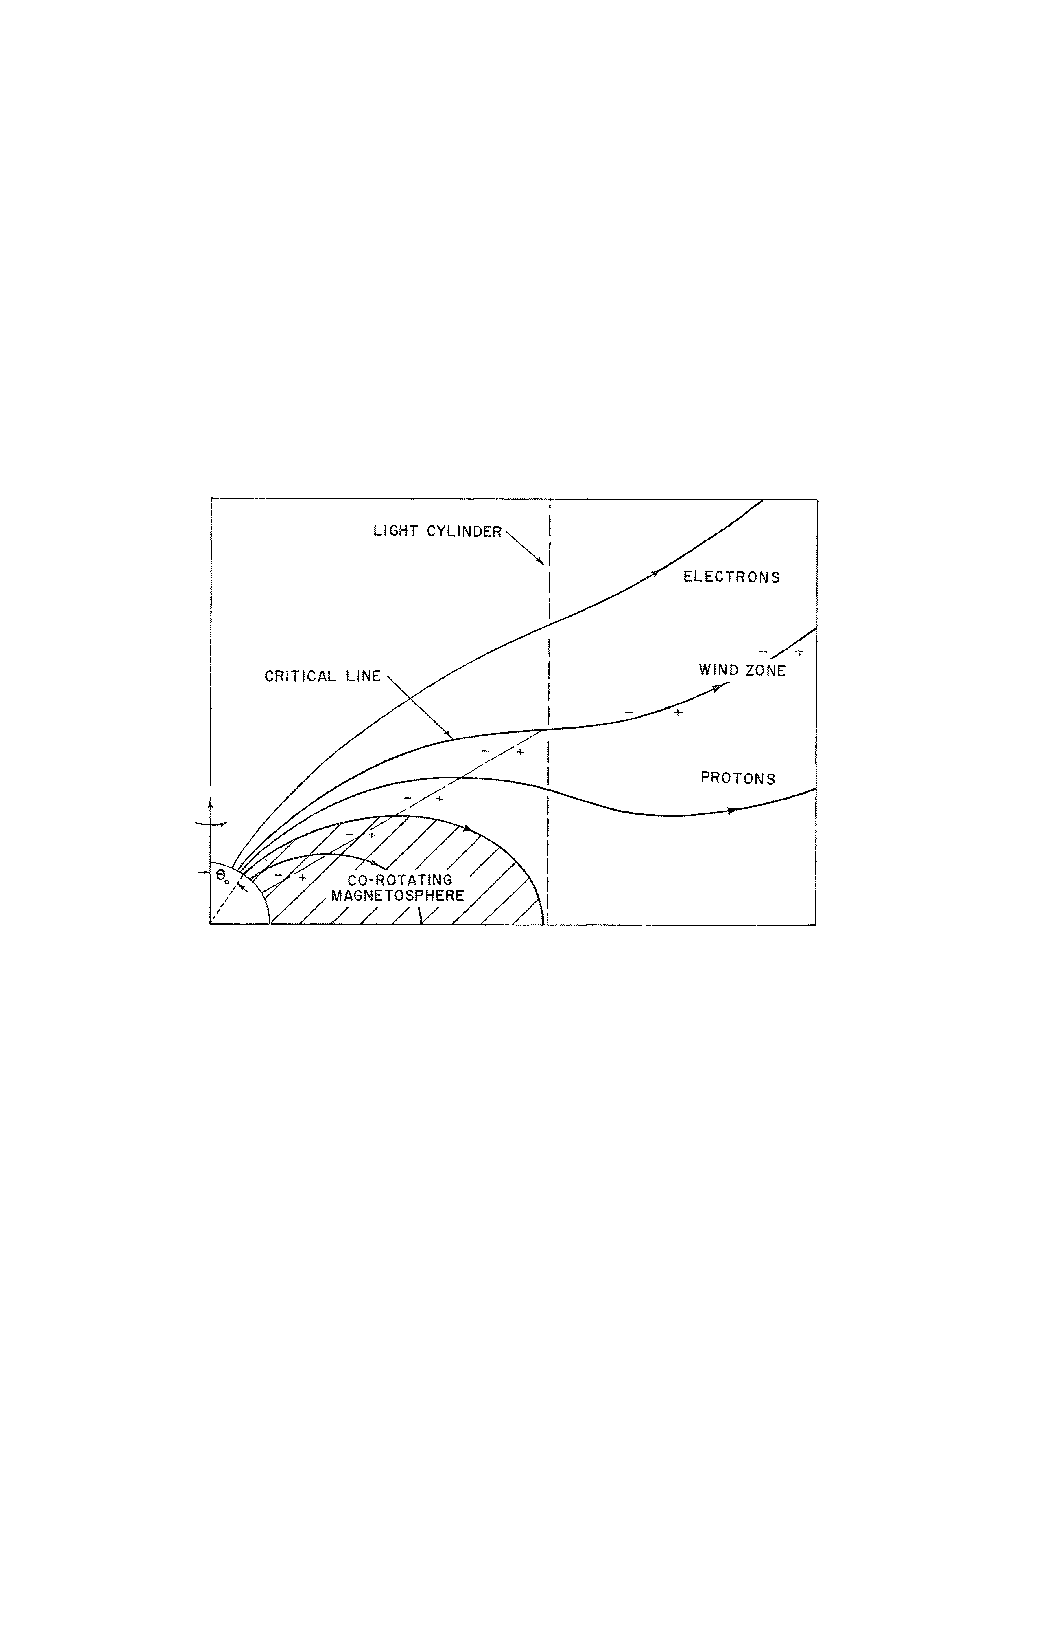
\includegraphics{chapters/pulsar_pwn_system/figures/pulsar_magnetosphere.pdf}
  \caption{The magnetosphere for a rotating pulsar.
  The pulsar is on the bottom left of the plot. This figure is
  from \cite{goldreich_1969_pulsar-electrodynamics}.}
  \figlabel{pulsar_magnetosphere}
\end{figure}

\figref{pulsar_magnetosphere} shows a schematic diagram of this
magnetosphere. It is commonly believed that the radio emission
from pulsars originates within 10\% of the light cylinder radius
\citep[see][and references therein]{kijak_2003a_radio-emission}

On the other hand, there is still much debate about the location
of the $\gamma$-ray emission.  Three locations have been proposed.
In the \ac{PC} model, the $\gamma$-ray emission arises from within one
stellar radius \citep{daugherty_1996a_gamma-ray-pulsars:}.  This model
was disfavored based upon the predicted $\gamma$-ray spectrum
\citep{abdo_2009b_fermi-large}.  In the \ac{OG} model,
$\gamma$-ray emission is predicted near the pulsar's light cylinder
\citep{cheng_1986a_energetic-radiation,romani_1996a_gamma-ray-pulsars:}.
Finally, in the \ac{TPC} model, the $\gamma$-ray emission
comes from an intermediate region in the pulsar magnetosphere
\citep{dyks_2003a_two-pole-caustic,muslimov_2004a_high-altitude-particle}
Much work has gone into comparing the \ac{TPC} and
\ac{OG} models in the context of detailed \ac{LAT}
observations of $\gamma$-ray pulsars \citep[See for
example][]{watters_2011a_galactic-population,romani_2011a_sub-luminous-gamma-ray}.
